\section{実験概要}
本研究で作成したドキュメントの有効性を確認するため, 津田沼チャレンジのコースを用いて自律移動実験を行った. 
実験では, ロボットが自律的にナビゲーションを実行し, 設定されたコースを完走できるかを確認することを目的とした. 

実験は, 作成者が2025年度版コースを対象に実施したものと, 学部3年生が2024年度版コースでドキュメントを参照して実施したものの2種類である. 
それぞれのコースを\figref{Fig:Course map of the Tsudanuma Challenge 2025}, \figref{Fig:Course map of the Tsudanuma Challenge 2024}に示す.
作成者の実験では, 走行地図の作成から自己位置推定および経路計画に関する各種パラメータの調整までを一貫して行った. 
一方, 学部3年生による実験では, 作成者がまとめたドキュメントを基に, 作成者が作成した地図を使用してナビゲーションの構築と調整を行った. 

実験に用いたロボットは本研究室で開発されているロボットORNE-box2\cite{井口颯人2023屋外自律移動ロボットプラットフォーム-orne}を使用した. 
その外観を\figref{Fig:ORNE-box2}に示す. 
また, ナビゲーションにはROS Navigation Stackを用いた. 
\begin{figure}[hbtp]
  \centering
 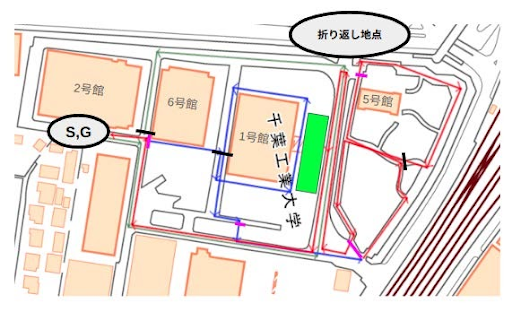
\includegraphics[keepaspectratio, scale=0.5]
      {images/2025tsudacha.png}
 \caption{Course map of the Tsudanuma Challenge 2025(souce: \cite{tsudachare})}
 \label{Fig:Course map of the Tsudanuma Challenge 2025}
\end{figure}
\begin{figure}[hbtp]
  \centering
 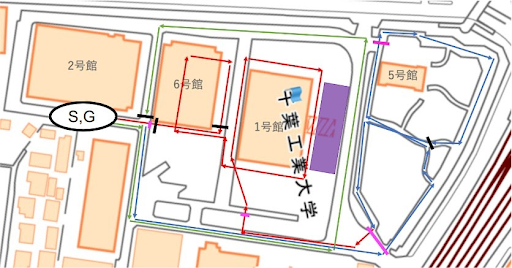
\includegraphics[keepaspectratio, scale=0.5]
      {images/2024tsudacha.png}
 \caption{Course map of the Tsudanuma Challenge 2024(souce: \cite{tsudachare})}
 \label{Fig:Course map of the Tsudanuma Challenge 2024}
\end{figure}
\begin{figure}[hbtp]
  \centering
 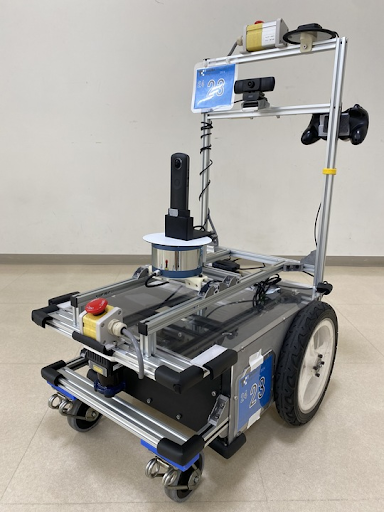
\includegraphics[keepaspectratio, scale=0.3]
      {images/box2.png}
 \caption{ORNE-box2}
 \label{Fig:ORNE-box2}
\end{figure}





\section{実験結果}


\subsection{作成者による結果}


\subsection{学部3年生による結果}